\subsection{Крайно произведение}
\label{subsect:domains:product}
\index{област на Скот!крайно произведение}
\marginpar{\cite[стр. 125]{winskel}}

Нека $\A$ и $\B$ са области на Скот.
Тогава $\A \times \B \df (A \times B,\sqsubseteq,\bot)$, където
\begin{itemize}
\item
  $A \times B = \{\pair{a,b} \mid a \in A\ \&\ b \in B\}$;
\item
  $\pair{a,b} \sqsubseteq \pair{a',b'} \iff a \sqsubseteq^\A a'\ \&\ b \sqsubseteq^\B b'$;
\item
  $\bot = \pair{\bot^\A,\bot^\B}$.
\end{itemize}

\begin{framed}
  \begin{proposition}
    \label{pr:cartesian}
    Ако $\A,\B$ са области на Скот, то $\A \times \B$ е област на Скот.
  \end{proposition}  
\end{framed}
\begin{hint}
  Лесно се съобразява, че $\sqsubseteq$ е частична наредба и че $\bot$ е най-малкият елемент.
  Да разгледаме една верига $\{\pair{a_i,b_i}\}^\infty_{i=1}$ в $\A \times \B$.
  Лесно се вижда, че
  \[\bigsqcup_i\pair{a_i,b_i} = \pair{\bigsqcup_ia_i,\bigsqcup_ib_i}.\]
  \begin{itemize}
  \item
    За произволен елемент $\pair{a_i,b_i}$ от веригата е ясно, че $a_i \sqsubseteq^\A \bigsqcup_ia_i$ и $b_i \sqsubseteq^\B \bigsqcup_i b_i$.
    Следователно, $\pair{\bigsqcup_ia_i,\bigsqcup_ib_i}$ е горна граница на веригата.
  \item
    Нека $\pair{c,d}$ е горна граница на веригата, т.е. за всяко $i$,
    $a_i \sqsubseteq^\A c$ и $b_i \sqsubseteq^\B d$.
    Но тогава $c$ е горна граница на веригата $\chain{a}{i}$ и следователно $\bigsqcup_ia_i \sqsubseteq^\A c$.
    Също така, $d$ е горна граница на веригата $\chain{b}{i}$ и следователно $\bigsqcup_i b_i \sqsubseteq^\B d$.
    Заключаваме, че $\pair{\bigsqcup_ia_i,\bigsqcup_ib_i} \sqsubseteq \pair{c,d}$, т.е. $\pair{\bigsqcup_ia_i,\bigsqcup_ib_i}$
    е точна горна граница на веригата.
  \end{itemize}
\end{hint}

Нека $\A_1,\dots,\A_n$, $n \geq 2$, са области на Скот. Дефинираме 
$\prod^n_{i=1}\A_i = (A, \sqsubseteq, \bot)$ по следния начин:
\begin{itemize}
\item
  Ако $n = 2$, то $\prod^2_{i=1} \A_i \df \A_1 \times \A_2$.
\item
  Ако $n > 2$, то $\prod^n_{i=1} \A_i \df (\prod^{n-1}_{i=1}\A_i) \times \A_n$.
\end{itemize}

Използвайки \Prop{cartesian}, лесно се съобразява следното твърдение.
\begin{proposition}
  Ако $\A_1,\dots,\A_n$, $n \geq 2$, са области на Скот, то $\prod^n_{i=1}\A_i$ е област на Скот.
\end{proposition}

\begin{framed}
  \begin{figure}[H]
    \centering
    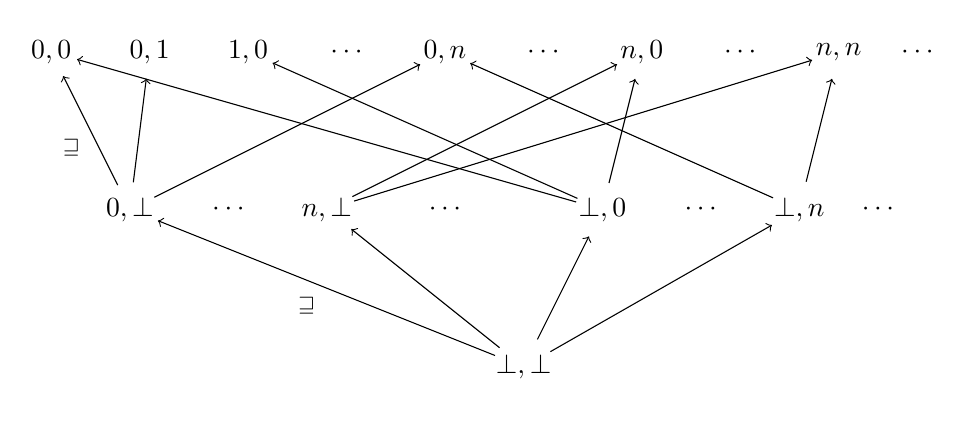
\begin{tikzpicture}[shorten >=1pt,->]
      \tikzstyle{vertex}=[circle,minimum size=17pt,inner sep=0pt]
      
      \node[vertex] (bot) at (5,-1) {$\pair{\bot,\bot}$};
      
      \node[vertex] (0b) at (0,1) {$\pair{0,\bot}$};
      \node[vertex] (db) at (1.25,1) {$\cdots$};
      \node[vertex] (nb) at (2.5,1) {$\pair{n,\bot}$};
      \node[vertex] (ddb) at (4,1) {$\cdots$};
      
      \node[vertex] (b0) at (6,1) {$\pair{\bot,0}$};
      \node[vertex] (bd) at (7.25,1) {$\cdots$};
      \node[vertex] (bn) at (8.5,1) {$\pair{\bot,n}$};
      \node[vertex] (bdd) at (9.5,1) {$\cdots$};
      
      \node[vertex] (00) at (-1,3) {$\pair{0,0}$};
      \node[vertex] (01) at (0.25,3) {$\pair{0,1}$};
      \node[vertex] (10) at (1.5,3) {$\pair{1,0}$};
      \node[vertex] (ddd) at (2.75,3) {$\cdots$};
      \node[vertex] (0n) at (4,3) {$\pair{0,n}$};
      \node[vertex] (dddd) at (5.25,3) {$\cdots$};
      \node[vertex] (n0) at (6.5,3) {$\pair{n,0}$};
      \node[vertex] (ddddd) at (7.75,3) {$\cdots$};
      \node[vertex] (nn) at (9,3) {$\pair{n,n}$};
      \node[vertex] (dddddd) at (10,3) {$\cdots$};

      \draw (bot) -- node[below left]{$\scriptstyle{\sqsupseteq}$} (0b);
      \draw (bot) -- (nb);
      \draw (bot) -- (b0);
      \draw (bot) -- (bn);

      \draw (0b) -- node[below left]{$\scriptstyle{\sqsupseteq}$} (00);
      \draw (0b) -- (01);
      \draw (0b) -- (0n);

      \draw (b0) -- (00);
      \draw (b0) -- (10);
      \draw (b0) -- (n0);
      \draw (nb) -- (n0);
      
      \draw (nb) -- (nn);
      \draw (bn) -- (0n);
      \draw (bn) -- (nn);

    \end{tikzpicture}    
    \caption{Графично представяне на част от $\sqsubseteq$ върху $\Nat^2_\bot$}
    \label{fig:flat-nat-2}
  \end{figure}
\end{framed}

Вижда се от \Fig{flat-nat-2}, че всяка верига в $\Nat^2_\bot$ има дължина най-много $3$.
Лесно се съобразява, че всяка верига в $\Nat^k_\bot$ има дължина най-много $k+1$.
Свойството, че всяка верига в $\Nat^k_\bot$ има само краен брой различни члена
ще се окаже важно по-нататък. Сега ще въведем понятие, което описва това свойство в произволна област на Скот.
\marginpar{ $\Nat^k_\bot = \underbrace{\Nat_\bot \times \cdots \times\Nat_\bot}_{k}$}

Нека $\A$ е област на Скот и да разгледаме една верига $\chain{a}{n}$ в $\A$.
Ще казваме, че $\chain{a}{n}$ се {\bf стабилизира}, ако съществува индекс $n_0$, за който
\[(\forall n \geq n_0)[a_{n_0} = a_{n}],\]
т.е.
\[a_0 \sqsubseteq a_1 \sqsubseteq a_2 \sqsubseteq \cdots \sqsubseteq a_{n_0} = a_{n_0+1} = a_{n_0+2} = \cdots\]
От казаното по-горе следва, че всяка растяща верига в $\Nat^k_\bot$ се стабилизира.

\begin{remark}
  Едни от основните области на Скот, които ще разглеждаме при дефинирането на денотационната семантика
  ще бъдат $\Nat_\bot$ и $\Nat^k_\bot$.
\end{remark}


%%% Local Variables:
%%% mode: latex
%%% TeX-master: "../sep"
%%% End:
